\documentclass[11pt,a4paper]{article}
\usepackage[utf8]{inputenc}
\usepackage[T1]{fontenc}
\usepackage{lmodern}
\usepackage{textcomp}
\usepackage{amsmath,amssymb}
\usepackage{graphicx}
\usepackage{booktabs}
\usepackage{longtable}
\usepackage{array}
\usepackage{listings}
\usepackage{xcolor}
\usepackage[margin=1in]{geometry}
\usepackage{float}
\usepackage[hidelinks,breaklinks]{hyperref}
\usepackage{microtype}
\setlength{\parskip}{4pt}
\lstset{basicstyle=\ttfamily\scriptsize,breaklines=true,breakatwhitespace=false,
  postbreak=\mbox{\textcolor{gray}{$\hookrightarrow$}\space},frame=single,
  framerule=0.3pt,rulecolor=\color{gray!60},columns=fullflexible,keepspaces=true,
  showstringspaces=false,numbers=none,xleftmargin=4pt,xrightmargin=4pt,
  literate={\_}{{\_}}1}
\graphicspath{{figures/}}
\providecommand{\tightlist}{}
\title{BBN and X-ray Viability of keV Sterile-Neutrino Dark Matter: A Tool-Assisted 2024--2026 Survey}
\author{HEP-Genesis-Agent session record \\ \small Project: ramp-research-sterile-bbn-xray}
\date{2026-10-21}
\begin{document}
\maketitle
\noindent\textit{\small This document is an AI-generated account of an interactive session with the HEP-Genesis agent. Its text was written by a language model strictly from the session record; figures and numbers come only from tool results obtained during the session. The supplementary material and the transcript, generated alongside, document exactly what ran. Verify independently before use.}
\vspace{1em}

\begin{abstract}
We report a tool-assisted study of which regions of the sterile-neutrino dark-matter plane $(m_s,\sin^2 2\theta)$ survive the combination of Big Bang nucleosynthesis (BBN) and X-ray decay-line constraints. The literature component draws mainly on 2024--2026 arXiv work. BBN observables ($Y_p$, D/H, $\Delta N_{\rm eff}$) came from a sterile-neutrino server that uses a fit to the PRyMordial network and takes $\Delta N_{\rm eff}$ as its only BBN input.

A $100\times100$ Dodelson--Widrow (DW) scan over $m_s=1$--$100$ keV and $\sin^2 2\theta=10^{-15}$--$10^{-6}$ shows that BBN ($\Delta\chi^2>3.84$) excludes only large mixings, $\sin^2 2\theta\gtrsim 10^{-8}$--$3.5\times10^{-7}$. Along the server's $\Omega_s h^2=0.12$ line, $\Delta N_{\rm eff}=10^{-4}$--$1.1\times10^{-2}$ and $|\Delta\chi^2_{\rm BBN}|<0.15$. The overclosure bound is therefore 40--5000 times stronger than BBN, and BBN is not a useful constraint on keV dark matter in the absence of a lepton asymmetry. The server's radiative decay rate agrees with the standard formula to about 1.5\%.

Recent X-ray results provide the upper bounds on mixing. From the XRISM ten-cluster stack (arXiv:2510.24560) we derive $\sin^2 2\theta\lesssim4\times10^{-10}$ at 7.1 keV. NuSTAR limits, as quoted secondarily in arXiv:2507.18752, give $\lesssim10^{-12}$ at 6--40 keV, and INTEGRAL/SPI limits from the same source give $\lesssim3\times10^{-14}$ above 40 keV.

Non-resonant DW production is disfavoured as all of the dark matter. The verdict at 7.1 keV depends on the relic normalization, and the server's normalization differs from a published fit (arXiv:1705.01837) by a factor of 10--17 in mixing. The surviving region quoted in the literature, Shi--Fuller production with $L\gtrsim0.5$ at $m_s\gtrsim10$ keV and $\sin^2 2\theta\lesssim10^{-14}$, could not be tested with the available server. The synthesis table and several literature-derived limits remained contested by the session's critic.
\end{abstract}

\section{Introduction}
The user asked for a survey of recent (2024--2026) arXiv work on sterile-neutrino dark matter, and for BBN constraints to be combined with X-ray constraints to determine which $(m_s,\sin^2 2\theta)$ regions remain viable. BBN numbers ($Y_p$, D/H) were to come from the sterile-neutrino tools, and the answer was to be quantified with tool calls where possible.

The session organised this request into six lines of investigation:
\begin{enumerate}
\item BBN and relic-density constraints across the plane, from the sterile-neutrino server.
\item X-ray decay-line constraints from 2024--2026 limits, compared with server-computed line energies and rates.
\item A survey of 2024--2026 production mechanisms (Shi--Fuller resonant production with lepton asymmetry, reheating production, scalar decays), together with structure-formation bounds.
\item A synthesis into per-mechanism viability regions.
\item Re-extraction of contested literature numbers as verbatim quotes, with a limit table at $m_s=7.1$, 10, 20, 40 and 50 keV.
\item Resolution of a factor-3 discrepancy in the DW relic normalization, the thermal-equivalent mass $m_{\rm th}$ along the DW line, and a BBN robustness check that includes an electron-neutrino degeneracy $\xi_e$.
\end{enumerate}

The scope is limited to $m_s\lesssim100$ keV, the server's validity range. The session did not run any resonant-production Boltzmann calculation, any BBN calculation with $\xi_e$, or any analysis of X-ray data.

\section{Methods}
All computations ran locally; the dispatch reported local execution. Three tool families were used.

\paragraph{Literature tools.} The literature servers searched arXiv abstracts, retrieved metadata, downloaded full texts, read text chunks, extracted figures and recorded citations. Full texts were read for arXiv:2507.18752, arXiv:2405.17861, arXiv:2510.24560, arXiv:1705.01837 and arXiv:1702.08430. The text of astro-ph/0501562 was downloaded, but the mapping formula attributed to it was not quoted verbatim from it. Metadata only was obtained for arXiv:2502.17374, arXiv:2601.03346 and arXiv:2609.31340.

\paragraph{Sterile-neutrino server (\texttt{serve-sbbn.sh}).} Its self-description gives the following model and data choices.
\begin{itemize}
\item BBN abundances ($Y_p$, D/H, $^7$Li) come from a fit to the PRyMordial network, accurate to better than 0.3\%. The only BBN input is $\Delta N_{\rm eff}$.
\item The fit is valid for $N_{\rm eff}\in[2.044,6.044]$, $\omega_b h^2\in[0.019,0.0257]$, $\tau_n\in[866.4,890.4]$ s, and $m_s\lesssim100$ keV. Decay injection is not modelled for $m_s\ge1$ MeV.
\item The observational inputs are $Y_p=0.2449\pm0.004$ (Aver, Olive \& Skillman 2021), D/H $=(2.547\pm0.025)\times10^{-5}$ and Planck $N_{\rm eff}=2.99\pm0.17$.
\item A point is excluded if $\Delta\chi^2_{\rm BBN}>3.84$ relative to the Standard Model (SM).
\item Two mechanisms are available. In DW (non-resonant) mode, $\Delta N_{\rm eff}$ follows from the DW relic density. In Shi--Fuller (SF) mode, $\Delta N_{\rm eff}$ is a heuristic equal to $0.1\times$ the DW value, the relic density is a fitting formula in the lepton asymmetry $L$, $L$ is capped at 0.1, and $L$ is not fed into the BBN network.
\end{itemize}

The following server runs were made:
\begin{itemize}
\item a DW grid, $m_s=7.1,10,20,50$ keV $\times$ $\sin^2 2\theta=10^{-10},10^{-12},10^{-14}$;
\item a DW grid of 9 masses (1--100 keV) $\times$ 12 mixings ($10^{-12}$--$3\times10^{-7}$);
\item zipped DW grids located on the $\Omega_s h^2=0.12$ line;
\item a $100\times100$ DW scan, $m_s=1$--$100$ keV and $\sin^2 2\theta=10^{-15}$--$10^{-6}$, with its exclusion plot;
\item SF grids at $m_s=10,20,30$ keV with $L=10^{-3}$ and $0.1$;
\item the BBN-versus-$N_{\rm eff}$ impact plot;
\item a BEST short-baseline cross-check;
\item X-ray line predictions at (7.1 keV, $10^{-10}$), (20 keV, $10^{-12}$), (10 keV, $10^{-12}$) and (50 keV, $3\times10^{-14}$). X-ray fluxes are whole-halo with $f_{\rm DM}=1$ and no field-of-view cut.
\end{itemize}

\paragraph{Hand calculations.} Three analyses were done by hand rather than by tools.
\begin{itemize}
\item Inversion of the published DW fit.
\item The DW-to-thermal mapping $m_s=4.43\,{\rm keV}\,(m_{\rm th}/{\rm keV})^{4/3}$.
\item Linearised BBN $\chi^2$ bounds, using the server slopes ${\rm d}Y_p/{\rm d}N_{\rm eff}=0.0135$ and ${\rm d}({\rm D/H}\times10^5)/{\rm d}N_{\rm eff}=0.331$ about the server SM values. The joint fit used ${\rm d}Y_p/{\rm d}\xi_e=-0.25$.
\end{itemize}

\paragraph{Research board and supplement.} Findings, dead ends and critic verdicts were tracked on a research board. The full tool-call log and the code are in the supplement.

\section{Results}
\subsection{Literature survey}
Four 2025--2026 papers on production mechanisms were confirmed to exist by metadata lookup.
\begin{itemize}
\item Vogel, Garc\'ia Escudero, Froustey and Abazajian, arXiv:2507.18752. This paper revives Shi--Fuller production.
\item Gorbunov, Kalashnikov and Krugan, arXiv:2502.17374. This paper studies flavor-dependent lepton asymmetry.
\item Cline and Xu, arXiv:2601.03346. This paper studies cold sterile-neutrino dark matter from inflaton decays during reheating, with branching ratio ${\rm BR}\lesssim10^{-4}$.
\item Gorbunov and Kalashnikov, arXiv:2609.31340. This paper studies saturation of resonant production at high flavor asymmetry.
\end{itemize}

The full text of arXiv:2507.18752 was read. It states that ``lepton asymmetries $L\gtrsim0.5$ at high temperatures open significant viable parameter space in the $m_s\gtrsim10$ keV and $\sin^2(2\theta)\lesssim10^{-14}$ regime.'' It cites the following limits:
\begin{itemize}
\item NuSTAR: $\sin^2(2\theta)\lesssim10^{-12}$ in the 6--40 keV mass range.
\item INTEGRAL/SPI: ``exclude lifetimes below $\sim10^{20}$ s at 95\% CL [corresponding to $\sin^2(2\theta)\lesssim3\times10^{-14}$] in the $\gtrsim40$ keV mass regime.''
\item Structure formation: $m_{\rm th}>8.4$ keV (galaxy counts) and $m_{\rm th}>8.5$ keV (counts plus strong lensing), both at 95\% CL, and a Lyman-$\alpha$ preference $m_{\rm th}=4.1^{+33.3}_{-1.5}$ keV.
\end{itemize}
The paper also states that the original DW mechanism is ruled out as producing all of the dark matter.

The claims of arXiv:2502.17374, arXiv:2601.03346 and arXiv:2609.31340 are known only from their abstracts.
\begin{itemize}
\item arXiv:2502.17374: flavor asymmetries that cancel in active oscillations, more efficiently for inverted ordering, mitigate BBN limits. Asymmetry that disappears mid-production yields colder spectra that reopen lighter masses.
\item arXiv:2601.03346: reheating production reaches mixings small enough to evade X-ray limits.
\item arXiv:2609.31340: oscillation-induced redistribution saturates the abundance at large initial asymmetry.
\end{itemize}

On the X-ray side, two recent papers were found and read: the XRISM Resolve ten-cluster stack (arXiv:2510.24560) and the 11-year NuSTAR stray-light analysis (arXiv:2405.17861). Merle's 2017 review (arXiv:1702.08430) served only as older context.

A web snippet mentioned eROSITA eFEDS line limits over 1.8--18 keV. No citable arXiv identifier was found for it, so it was not used. In its initial survey summary, written before the server was used, the assistant cautioned that it had no BBN tool and that its BBN statements were abstract-level. That gap was closed in the subsequent waves.

\subsection{BBN versus the DW plane}
The DW scan of $10^4$ points flagged 1338 points as BBN-excluded and 4300 as overclosing ($\Omega_s h^2>0.12$). The largest BBN-allowed mixing at each mass is listed in Table~\ref{tab:bbn}, alongside the server's dark-matter line.

\begin{table}[h]
\centering
\begin{tabular}{lcc}
\toprule
$m_s$ (keV) & BBN-allowed max $\sin^2 2\theta$ & DW line ($\Omega_s h^2=0.12$, server) \\
\midrule
1 & $3.5\times10^{-7}$ & $8.7\times10^{-9}$ \\
3--3.7 & $1.2\times10^{-7}$ (3.7 keV) & $1.2\times10^{-9}$ (3 keV) \\
7--7.1 & $8.1\times10^{-8}$ & $2.55\times10^{-10}$ \\
10--13.5 & $4.3\times10^{-8}$ (13.5 keV) & $1.37\times10^{-10}$ (10 keV) \\
20 & -- & $3.9\times10^{-11}$ \\
50 & $1.5\times10^{-8}$ & $7.6\times10^{-12}$ \\
100 & $1\times10^{-8}$ & $2.2\times10^{-12}$ \\
\bottomrule
\end{tabular}
\caption{BBN-allowed upper mixing from the DW scan, and the server's DW dark-matter line. The line was also computed at 2 keV ($2.5\times10^{-9}$) and 5 keV ($4.8\times10^{-10}$).}
\label{tab:bbn}
\end{table}

Along the dark-matter line, $\Delta N_{\rm eff}=10^{-4}$--$1.1\times10^{-2}$ and $|\Delta\chi^2_{\rm BBN}|<0.15$. Overclosure is thus 40 times (1 keV) to about 5000 times (100 keV) more restrictive than BBN. The entire DW line, and everything below it, is BBN-allowed.

The benchmark grid at 7.1--50 keV and $10^{-14}$--$10^{-10}$ is consistent with this: no point was excluded, $\Delta N_{\rm eff}\le2.9\times10^{-3}$, and $|\Delta\chi^2|\le0.04$. The same grid gives the DW abundance at $10^{-10}$:
\begin{itemize}
\item $\Omega_s h^2=0.087$ at 10 keV;
\item $\Omega_s h^2=0.30$ at 20 keV, which overcloses;
\item $\Omega_s h^2=1.58$ at 50 keV, which overcloses.
\end{itemize}
At $10^{-12}$--$10^{-14}$ the DW abundance is $\Omega_s h^2\le0.016$.


\begin{figure}[H]
\centering
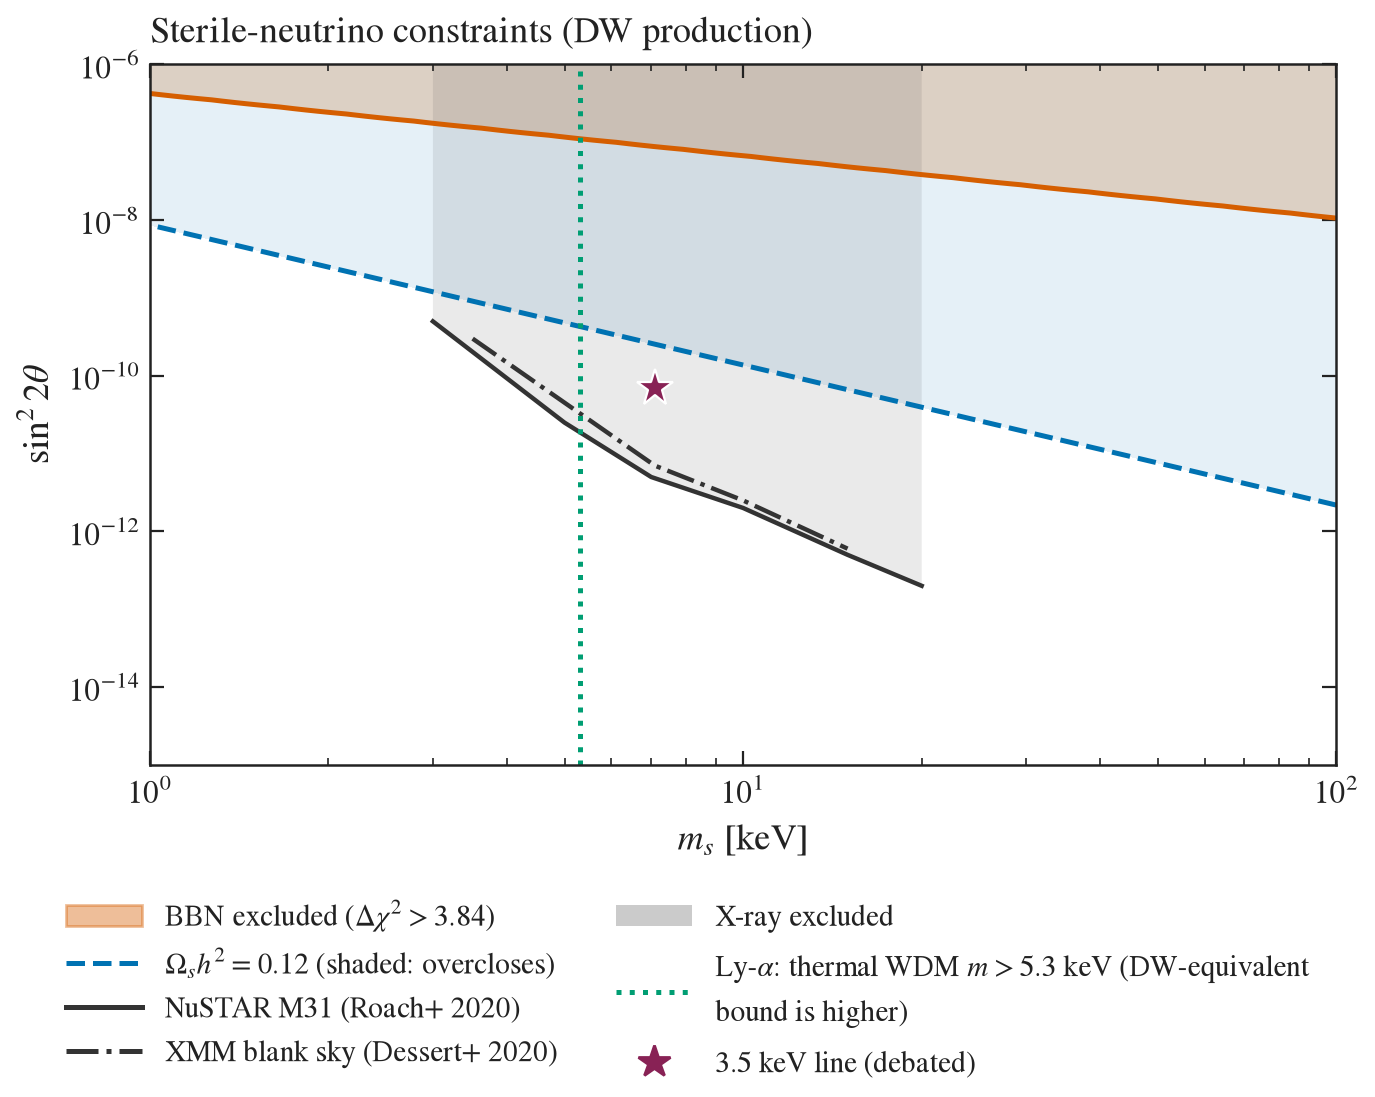
\includegraphics[width=0.85\textwidth,height=0.6\textheight,keepaspectratio]{fig-8.png}
\caption{exclusion\_scan\_DW\_dc7743.png Produced in this session by \texttt{plot\_sterile\_nu\_exclusion} on \textit{serve-sbbn.sh}.}
\label{fig:8}
\end{figure}



Figure~\ref{fig:8} shows the exclusion plane produced from this scan. The BBN-excluded band sits at large mixing, and the overclosure region lies well below it. This visualises the hierarchy in Table~\ref{tab:bbn}: for DW production the binding cosmological constraint is the abundance, not nucleosynthesis.

\paragraph{Representative BBN points.} Table~\ref{tab:points} lists server outputs at selected points, with deviations quoted against the brief's data ($Y_p=0.245\pm0.003$ and D/H $=(2.53\pm0.03)\times10^{-5}$).

\begin{table}[h]
\centering
\begin{tabular}{lccccc}
\toprule
Point & $\Delta N_{\rm eff}$ & $Y_p$ & D/H $\times10^5$ & $\Delta\chi^2$ & Verdict \\
\midrule
SM ($N_{\rm eff}=3.044$) & 0 & 0.246815 ($+0.6\sigma$) & 2.4433 ($-2.9\sigma$) & 0 & baseline\\
7.1 keV, $3\times10^{-10}$ & -- & 0.24684 & 2.4440 & $-0.024$ & allowed\\
1 keV, $3\times10^{-7}$ & 0.387 & 0.25193 ($+2.3\sigma$) & 2.5718 ($+1.4\sigma$) & $+0.44$ & allowed\\
10 keV, $10^{-7}$ & 0.813 & 0.25730 ($+4.1\sigma$) & 2.7145 ($+6.2\sigma$) & 13.4 & excluded\\
3 keV, $3\times10^{-7}$ & 0.931 & 0.25874 ($+4.6\sigma$) & 2.7540 ($+7.5\sigma$) & 19.3 & excluded\\
\bottomrule
\end{tabular}
\caption{Server BBN outputs at representative DW points.}
\label{tab:points}
\end{table}

The 1 keV point is allowed despite its $Y_p$ excess. The server's SM D/H lies below the data, so additional radiation improves the D/H fit and offsets the $Y_p$ penalty.


\begin{figure}[H]
\centering
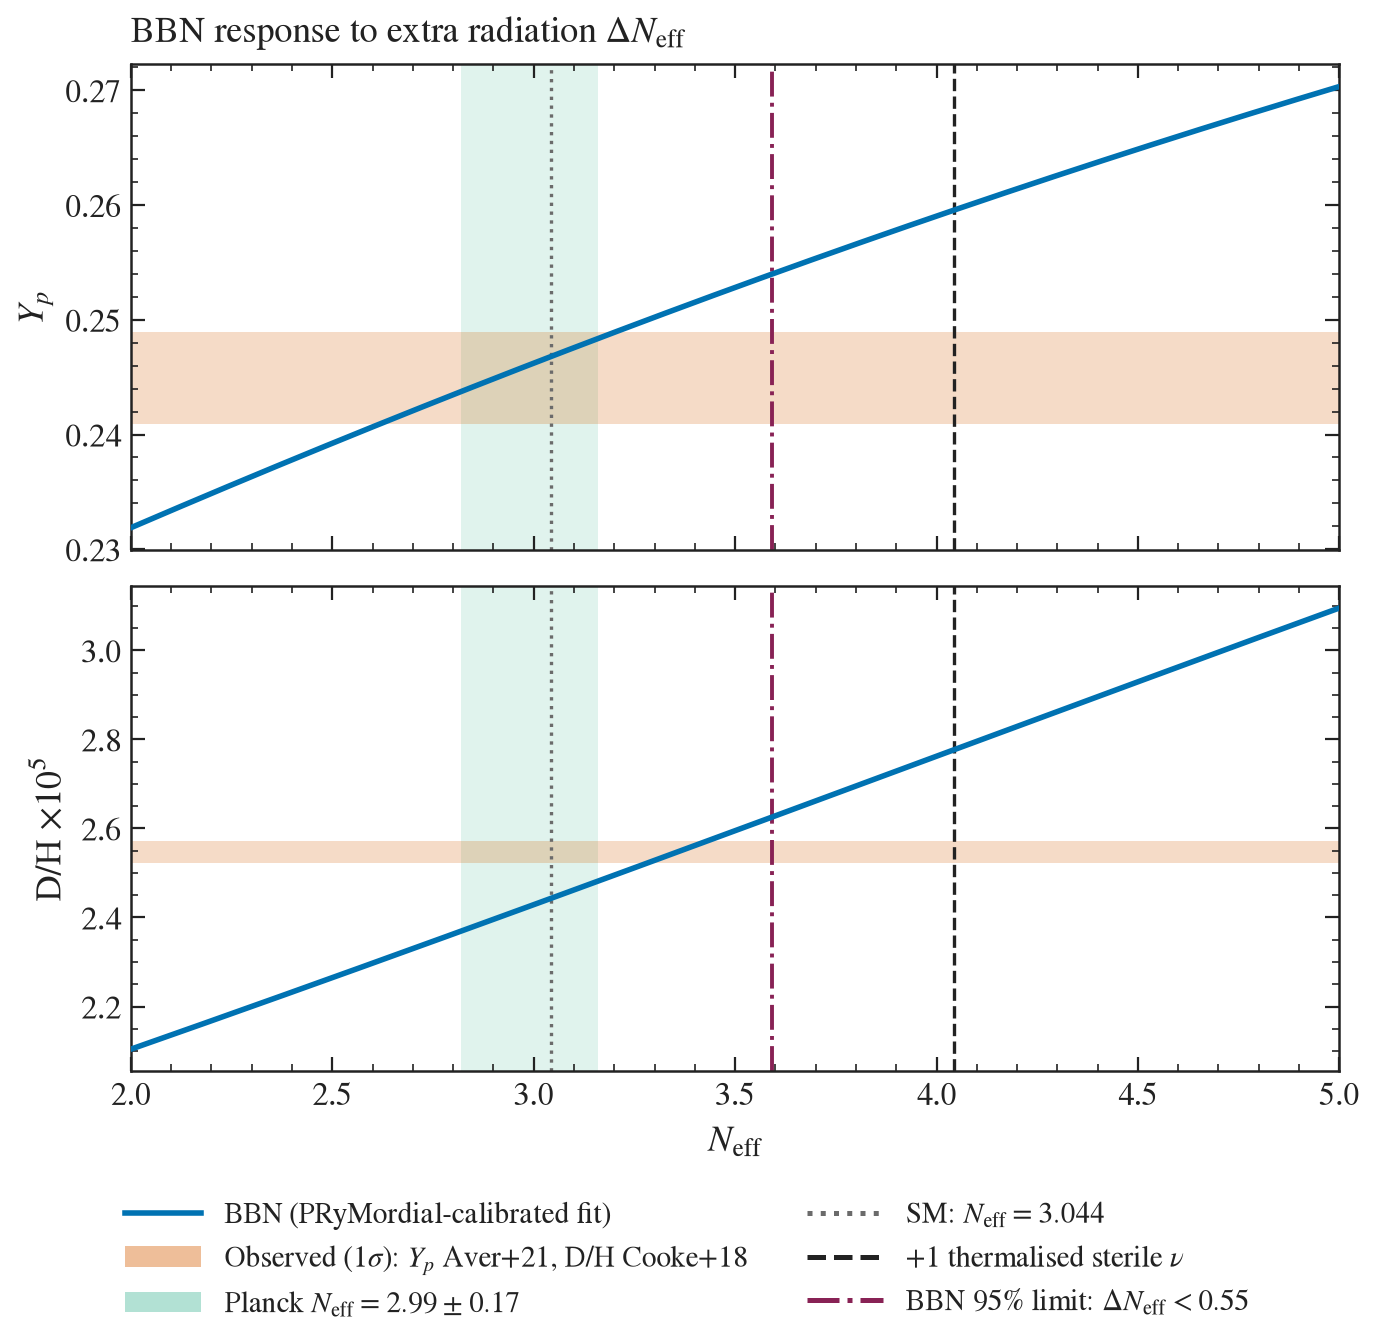
\includegraphics[width=0.85\textwidth,height=0.6\textheight,keepaspectratio]{fig-6.png}
\caption{bbn\_vs\_neff.png Produced in this session by \texttt{plot\_sterile\_nu\_bbn\_impact} on \textit{serve-sbbn.sh}.}
\label{fig:6}
\end{figure}



Figure~\ref{fig:6} shows the server's $Y_p$ and D/H as functions of $N_{\rm eff}$, with the observational bands. A fully thermalised sterile state ($N_{\rm eff}=4.044$) gives $Y_p=0.2596$ and D/H $=2.777\times10^{-5}$, which is $3.7\sigma$ above the observed $Y_p$. BBN alone limits $\Delta N_{\rm eff}<0.548$ at 95\%, with slopes ${\rm d}Y_p/{\rm d}N_{\rm eff}=0.01351$ and ${\rm d}({\rm D/H}\times10^5)/{\rm d}N_{\rm eff}=0.3308$.

The BEST cross-check ($m_s=1.14$ eV, $\sin^2 2\theta=0.42$) gave the following, although the critic had judged this check tangential to the keV question:
\begin{itemize}
\item $\Delta N_{\rm eff}=1$, $Y_p=0.25956$, $\Delta\chi^2=23.1$, so the point is excluded;
\item $6.2\sigma$ tension with Planck, and a projected $33\sigma$ at CMB-S4;
\item $\Omega_s h^2=29.3$.
\end{itemize}

\subsection{BBN robustness: data baseline and $\xi_e$}
These bounds come from a linearised hand analysis, not from server runs. Table~\ref{tab:rob} gives 95\% upper limits on $\Delta N_{\rm eff}$ for $\Delta\chi^2=3.84$ relative to the SM; values in brackets are relative to the best fit.

\begin{table}[h]
\centering
\begin{tabular}{lccc}
\toprule
Data & $Y_p$ only & D/H only & combined\\
\midrule
Brief ($0.245\pm0.003$; $2.53\pm0.03$) & 0.32 & 0.58 [0.44] & 0.47 [0.37]\\
Server ($0.2449\pm0.004$; $2.547\pm0.025$) & 0.46 & 0.66 [0.46] & 0.61 [0.43]\\
\bottomrule
\end{tabular}
\caption{Linearised 95\% bounds on $\Delta N_{\rm eff}$. The server's own reported limit is 0.548.}
\label{tab:rob}
\end{table}

The server's SM D/H lies $2.9\sigma$ (brief data) to $4.1\sigma$ (server data) below the observations. Because of this, D/H alone prefers $\Delta N_{\rm eff}\approx0.26$--$0.31$, and the bound shifts by 0.1--0.2 depending on the baseline.

The joint $(\Delta N_{\rm eff},\xi_e)$ fit used ${\rm d}Y_p/{\rm d}\xi_e=-0.25$, assumed D/H independent of $\xi_e$, and applied two degrees of freedom ($\Delta\chi^2=5.99$).
\begin{itemize}
\item Brief data: $\Delta N_{\rm eff}\in[0.04,0.48]$ with $\xi_e=0.0073+0.054\,\Delta N_{\rm eff}\pm0.029$.
\item Server data: $\Delta N_{\rm eff}\in[0.13,0.50]$ with $\xi_e=0.0077+0.054\,\Delta N_{\rm eff}\pm0.039$.
\end{itemize}
Overall this implies $|\xi_e|\lesssim0.03$--$0.06$. A positive $\xi_e\approx0.03$ compensates $\Delta N_{\rm eff}\approx0.5$ in $Y_p$. Neglecting ${\rm d(D/H)}/{\rm d}\xi_e$ biases this contour.

\subsection{Shi--Fuller runs with the server}
SF runs at $m_s=10,20,30$ keV with $\sin^2 2\theta=10^{-14}$ gave $\Delta N_{\rm eff}\sim10^{-8}$ and $\Delta\chi^2_{\rm BBN}=0$. At 20 keV the outputs were $Y_p=0.24682$ and D/H $=2.4433\times10^{-5}$. The relic abundance $\Omega_s h^2$ at the three masses was:
\begin{itemize}
\item $L=10^{-3}$: 0.122, 0.490 and 1.10;
\item $L=0.1$: 1.22, 4.90 and 11.0.
\end{itemize}
All of these points were flagged as overclosing.

These runs do not test arXiv:2507.18752, for four reasons:
\begin{itemize}
\item $L$ is capped at 0.1, while the paper requires $L\gtrsim0.5$;
\item the SF $\Delta N_{\rm eff}$ is a heuristic;
\item $\xi_e$ does not enter $Y_p$;
\item the SF abundance is a fitting formula, not a Boltzmann calculation.
\end{itemize}
The BBN ``allowed'' verdict here is trivial, and the overclosure flags do not contradict the paper.

\subsection{X-ray decay rate and limits}
The server's rate agrees with $\Gamma=1.38\times10^{-32}\,{\rm s^{-1}}\,(\sin^2 2\theta/10^{-10})(m_s/{\rm keV})^5$ to about 1.5\%.
\begin{itemize}
\item At 7.1 keV and $10^{-10}$: $2.46\times10^{-28}$ s$^{-1}$ (formula $2.49\times10^{-28}$), with $E_\gamma=3.55$ keV and lifetime $4.07\times10^{27}$ s.
\item At 20 keV and $10^{-12}$: $4.36\times10^{-28}$ s$^{-1}$ (formula $4.42\times10^{-28}$), with $E_\gamma=10$ keV.
\end{itemize}
Eq.~2 of arXiv:2405.17861, $\Gamma_\gamma=1.36\times10^{-22}(m_s/1\,{\rm keV})^5\sin^2 2\theta$ s$^{-1}$, is consistent with this formula.

The whole-halo fluxes at (7.1 keV, $10^{-10}$) are 4.68 ph s$^{-1}$ cm$^{-2}$ for the Milky Way centre, $6.89\times10^{-4}$ for M31 and $3.55\times10^{-5}$ for Perseus. The server's built-in limits, NuSTAR M31 (Roach+ 2020) and XMM blank sky (Dessert+ 2020), exclude both test points.

\paragraph{XRISM.} The XRISM Resolve stack (arXiv:2510.24560) combines 3.75 Ms on ten clusters over 2.5--15 keV and detects no unidentified lines. Its $3\sigma$ limit at $m_s\sim7.1$ keV is $\Gamma\sim1.0\times10^{-27}$ s$^{-1}$. This is ``3$-$4 times lower than'' the Hitomi Perseus limit ``but still 5 times higher than the XMM-Newton detection reported by Bulbul et al.\ (2014),'' so the 3.55 keV line is constrained but not excluded. Scaling the server rate gives $\sin^2 2\theta\lesssim4\times10^{-10}$; this conversion is the session's own, not a quoted value.

\paragraph{NuSTAR.} arXiv:2405.17861 sets 95\% limits for $m_s=6$--40 keV. It states that the limits ``reach the bottom edge of theoretical predictions,'' that observed limits are stronger than expected at 8--9 and 23--25 keV, and that there is an instrumental excess at 40 keV. Numerical limit values could not be read from the paper: Fig.~3 was absent from the HTML rendering, and the downloaded Fig.~1 image could not be digitised.


\begin{figure}[H]
\centering
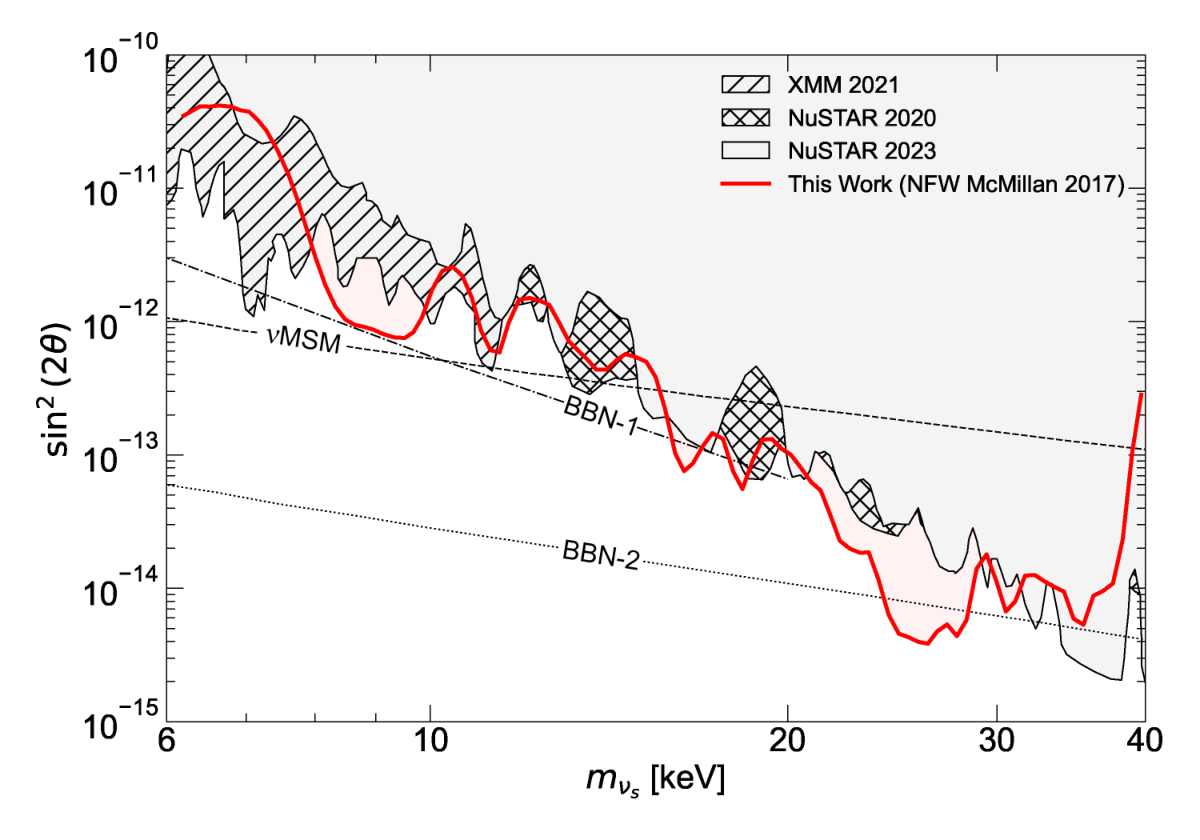
\includegraphics[width=0.85\textwidth,height=0.6\textheight,keepaspectratio]{fig-15.png}
\caption{Figure 1: 95\% upper limits on sin\textasciicircum{}\{2\}(2\textbackslash{}theta) derived from the NuSTAR unfocused stray light spectrum for reference profile [15] along with some previous constraints [9, NuSTAR 2020, 2023:], [16, XMM 2021:] and updated theoretical lower bounds [17, 18, 19]. Note that the borderline excess at 40 keV is the known instrumental effect caused by absorbed stray light [20, 21, 22]. [arXiv:2405.17861] Reproduced from arXiv:2405.17861 (extracted with \texttt{get\_paper\_figures}).}
\label{fig:15}
\end{figure}



Figure~\ref{fig:15} reproduces Fig.~1 of arXiv:2405.17861. According to its caption, it shows the 95\% upper limits on $\sin^2(2\theta)$ from the NuSTAR unfocused stray-light spectrum for the reference profile, together with earlier NuSTAR and XMM constraints and updated theoretical lower bounds. It attributes the borderline excess at 40 keV to absorbed stray light. No number in this report was read from the figure. It documents qualitatively that the 6--40 keV NuSTAR limits approach the theoretical lower bounds.

\paragraph{Limit table.} The X-ray limit table assembled in the session is given in Table~\ref{tab:xray}. It was contested by the critic, because only the XRISM entry derives from a primary source; the NuSTAR and SPI values are secondary quotes from arXiv:2507.18752.

\begin{table}[h]
\centering
\begin{tabular}{lll}
\toprule
$m_s$ & Limit on $\sin^2 2\theta$ & Server line-tool check\\
\midrule
7.1 keV & XRISM $\lesssim4\times10^{-10}$ (3$\sigma$, derived); NuSTAR $\lesssim10^{-12}$ & $10^{-10}$ excluded by built-in tables\\
10 keV & NuSTAR $\lesssim10^{-12}$ & at $10^{-12}$: $\Gamma=1.36\times10^{-29}$ s$^{-1}$, $E=5$ keV; not excluded\\
20 keV & NuSTAR $\lesssim10^{-12}$ & $10^{-12}$ excluded (built-in NuSTAR M31 table)\\
40 keV & NuSTAR upper edge; SPI $\lesssim3\times10^{-14}$ above & --\\
50 keV & SPI $\lesssim3\times10^{-14}$ & at $3\times10^{-14}$: $\Gamma=1.28\times10^{-27}$ s$^{-1}$, $E=25$ keV; not excluded\\
\bottomrule
\end{tabular}
\caption{X-ray limits versus mass (95\% CL unless noted). Contested.}
\label{tab:xray}
\end{table}

The session flagged an inconsistency in the SPI entry. The quote equates ``lifetimes below $\sim10^{20}$ s'' with $\sin^2 2\theta\lesssim3\times10^{-14}$, but the server gives a lifetime of $7.84\times10^{26}$ s ($2.48\times10^{19}$ yr) at 50 keV and that mixing. The assistant noted that the year-valued lifetime is close to $10^{20}$; the record does not resolve the discrepancy further.

\subsection{DW normalization and structure formation}
The server's DW abundance scales as $\Omega_s h^2=0.1(\sin^2 2\theta/10^{-9})(m_s/3\,{\rm keV})^{1.8}$. This was checked at three points: 3 keV and $10^{-9}$ gives 0.100; 10 keV and $10^{-9}$ gives 0.873, a ratio of 8.73 that equals $(10/3)^{1.8}$; and 1 keV and $10^{-8}$ gives 0.138. The exponent matches the brief's formula, but the normalization corresponds to three times smaller mixing on the dark-matter line.

The published fit in the Abazajian review (arXiv:1705.01837, Eq.~37) is
\[
m_s\sim3.40\,{\rm keV}\,(\sin^2 2\theta/10^{-8})^{-0.615}(\Omega_{\rm DM}/0.26)^{0.5}\times0.527\,{\rm erfc}[-1.15(T_{\rm QCD}/170\,{\rm MeV})^{2.15}].
\]
Inverting it by hand gives the dark-matter line at $\sin^2 2\theta\sim1.23\times10^{-8}$ (3 keV), $3.0\times10^{-9}$ (7.1 keV), $1.73\times10^{-9}$ (10 keV), $5.6\times10^{-10}$ (20 keV) and $1.26\times10^{-10}$ (50 keV). Varying $T_{\rm QCD}$ over 150--200 MeV shifts these by roughly $+10\%/-7\%$. Compared with the server line, the published fit requires 10--17 times more mixing; compared with the brief's formula, 3.4--5.5 times more.

At 7.1 keV the DW verdict against the XRISM-derived limit therefore depends on the normalization:
\begin{itemize}
\item the server line ($2.55\times10^{-10}$) survives;
\item the brief's line ($7.65\times10^{-10}$) is excluded;
\item the published line ($3.0\times10^{-9}$) is excluded by about a factor of 7.5.
\end{itemize}
The assistant concluded that server-based DW statements are not conservative. This conclusion and the normalization comparison were both marked contested.

\paragraph{Thermal-equivalent mass.} The mapping $m_s=4.43\,{\rm keV}\,(m_{\rm th}/{\rm keV})^{4/3}$ was attributed to Viel et al.\ (astro-ph/0501562), but was not quoted verbatim from that paper. It gives $m_{\rm th}=0.75$, 1.42, 1.84, 3.10 and 6.16 keV at $m_s=3$, 7.1, 10, 20 and 50 keV. Lyman-$\alpha$ bounds of $m_{\rm th}>4$ (6) keV then require $m_s>28$ (48) keV, and satellite counts ($m_{\rm th}>8.4$ keV) require $m_s>76$ keV. At those masses the DW line, about $3\times10^{-10}$ (published) or about $10^{-11}$ (server), lies far above the NuSTAR and SPI ceilings. On this basis DW is excluded by the combination of structure formation and X-ray limits regardless of normalization.

\subsection{Per-mechanism viability}
The final viability table (contested) reads as follows.
\begin{itemize}
\item \textbf{DW.} Not viable as all of the dark matter. The binding constraints are X-ray limits combined with structure formation; BBN is non-binding, with $\Delta\chi^2<0.15$ along the line.
\item \textbf{Shi--Fuller with $L\gtrsim0.5$ above 20 MeV.} Quoted as viable at $m_s\gtrsim10$ keV and $\sin^2 2\theta\lesssim10^{-14}$, below the NuSTAR and SPI ceilings. This rests on arXiv:2507.18752 and was not tool-verified.
\item \textbf{Flavor-dependent asymmetry.} Lower mixings and lighter masses are reopened (arXiv:2502.17374, abstract only).
\item \textbf{Large-$L$ saturation.} This acts as an additional constraint on resonant production (arXiv:2609.31340, abstract only).
\item \textbf{Reheating production.} Mixings below the X-ray limits are reached with ${\rm BR}\lesssim10^{-4}$ (arXiv:2601.03346, abstract only).
\end{itemize}

\section{Discussion}
The robust computational result is negative but important. For keV sterile neutrinos without lepton asymmetry, the extra radiation on and below the DW dark-matter line is $\Delta N_{\rm eff}\lesssim10^{-2}$. $Y_p$ and D/H then cannot be distinguished from standard BBN, and BBN carries essentially no constraining power where dark matter lives. This was the critic's expectation at the planning stage, and the scan confirmed it quantitatively. BBN becomes relevant to sterile-neutrino dark matter only through the lepton asymmetry needed for resonant production. That effect the server cannot model, because $\xi_e$ is not an input.

The linearised robustness check shows that the BBN bound on $\Delta N_{\rm eff}$ shifts by 0.1--0.2 between data choices. It also shows that the low SM D/H of the server (2.9--4.1$\sigma$ below the data) mildly favours extra radiation. The session raised, without resolving, whether this low D/H reflects a nuclear-rate choice that biases the server's bounds.

Several tensions limit the strength of the X-ray synthesis.
\begin{itemize}
\item The server's DW normalization disagrees with the published fit by an order of magnitude, so the 7.1 keV verdict flips between normalizations.
\item The NuSTAR limits could not be extracted from the primary paper. The per-mass entries rest on a summary value of $\lesssim10^{-12}$ quoted in arXiv:2507.18752.
\item The server's own NuSTAR M31 table excludes $10^{-12}$ at 20 keV, which indicates that the summary value is not uniformly representative.
\item The SPI lifetime--mixing correspondence is internally inconsistent with the computed lifetime.
\item The DW-to-thermal mapping was not verified verbatim.
\end{itemize}

The critic left the following findings contested: the arXiv:2507.18752 extraction (later re-supported verbatim), the mechanism map, the XRISM conversion (later re-supported verbatim), the NuSTAR reading, the X-ray limit table, the final viability table, the normalization comparison and the 7.1 keV verdict. The critic's final verdict on the report was ``revise.''

Two literature searches were dead ends. Neither search tool returned a 2024--2026 eROSITA line-search paper, and a targeted search found no primary 2024+ INTEGRAL/SPI line limit at $m_s\ge40$ keV. The eROSITA eFEDS statement therefore remained an uncited web snippet, and the SPI entry depends wholly on a secondary quote.

\section{Conclusions}
Established with tools:
\begin{itemize}
\item BBN excludes DW sterile neutrinos only above $\sin^2 2\theta\sim10^{-8}$--$3.5\times10^{-7}$ over 1--100 keV. This is 40--5000 times weaker than overclosure, and the DW dark-matter line is BBN-allowed with $|\Delta\chi^2|<0.15$.
\item The server's BBN-only limit is $\Delta N_{\rm eff}<0.548$; linearised alternatives span 0.32--0.66 depending on data and probe.
\item The server's radiative rate is accurate to about 1.5\%.
\end{itemize}

Supported by the literature but partially contested:
\begin{itemize}
\item DW production cannot be all of the dark matter once X-ray limits and structure formation are combined.
\item The surviving region requires very small mixing, about $\lesssim10^{-14}$ at $m_s\gtrsim10$ keV for Shi--Fuller production with $L\gtrsim0.5$, or non-oscillation production. Neither was tested numerically.
\end{itemize}

Open questions raised in the session:
\begin{itemize}
\item a Shi--Fuller BBN test requiring a code that accepts $\xi_e$ (PRIMAT, AlterBBN, or PRyMordial with $\xi$);
\item numerical NuSTAR stray-light limits at 7, 10 and 20 keV, and a 50 keV limit from SPI or the NuSTAR Galactic Centre analysis;
\item whether the server's DW relic formula should be replaced by the Abazajian fit;
\item whether the server's SM D/H biases its $\Delta N_{\rm eff}$ bounds.
\end{itemize}

\section*{References}
\begin{itemize}
\item arXiv:2507.18752 --- C.~M.~Vogel, H.~Garc\'ia Escudero, J.~Froustey, K.~N.~Abazajian, ``Return of the Lepton Number: Sterile Neutrino Dark Matter Production and the Revival of the Shi-Fuller Mechanism'' (2025).
\item arXiv:2502.17374 --- D.~Gorbunov, D.~Kalashnikov, G.~Krugan, ``Playing with lepton asymmetry at the resonant production of sterile neutrino dark matter'' (2025).
\item arXiv:2601.03346 --- J.~M.~Cline, Y.~Xu, ``Sterile Neutrino Dark Matter as a Probe of Inflationary Reheating'' (2026).
\item arXiv:2609.31340 --- D.~Gorbunov, D.~Kalashnikov, ``Natural Saturation Of The Sterile Neutrino Dark Matter Resonant Production By a High Lepton Flavor Asymmetry In Primordial Plasma'' (2026).
\item arXiv:2510.24560 --- XRISM Collaboration, ``XRISM constraints on unidentified X-ray emission lines, including the 3.5 keV line, in the stacked spectrum of ten galaxy clusters'' (2025).
\item arXiv:2405.17861 --- R.~A.~Krivonos, V.~V.~Barinov, A.~A.~Mukhin, D.~S.~Gorbunov, ``Strong limits on keV-scale galactic sterile neutrino dark matter with stray light from NuSTAR after 11 years of operation'' (2024).
\item arXiv:1705.01837 --- Abazajian, ``Sterile neutrinos in cosmology.''
\item astro-ph/0501562 --- Viel et al., ``Constraining Warm Dark Matter candidates including sterile neutrinos and light gravitinos with WMAP and the Lyman-alpha forest'' (2005).
\item arXiv:1702.08430 --- A.~Merle, ``keV sterile neutrino Dark Matter'' (2017).
\end{itemize}

\section*{Data and code availability}
All outputs of this session are collected in the project folder \href{file:///Users/nramachandra/hep-genesis-testing/projects/ramp-research-sterile-bbn-xray}{\texttt{/\allowbreak{}Users/\allowbreak{}nramachandra/\allowbreak{}hep-genesis-testing/\allowbreak{}projects/\allowbreak{}ramp-research-sterile-bbn-xray}}.
The session produced 14 data files; the supplement lists them.
Full documentation of how these results were obtained is in the supplementary material (\texttt{supplement.pdf}: implementation details, the tool-call log, the research board with every finding and its evidence, figures not shown here, and the code index) and the verbatim transcript (\texttt{transcript.pdf}), generated alongside this report.


\end{document}
